\documentclass[12pt,a4paper]{report}

\usepackage[utf8]{inputenc}
\usepackage[T1]{fontenc}
\usepackage[french]{babel}
\usepackage{graphicx}
\usepackage{geometry}
\usepackage{xcolor}
\usepackage{fancyhdr}
\usepackage{titlesec}
\usepackage{tocloft}
\usepackage{pageslts}
\usepackage[hidelinks]{hyperref}

\geometry{margin=2.5cm}

\definecolor{orangeil}{RGB}{230,120,20}

% =========================
% Header / Footer (partout)
% =========================
\pagestyle{fancy}
\fancyhf{}
\fancyhead[C]{\textcolor{orangeil}{Rapport Projet IL S6}}
\fancyfoot[C]{\thepage}
\renewcommand{\headrulewidth}{0.4pt}
\renewcommand{\footrulewidth}{0.4pt}

\fancypagestyle{plain}{
  \fancyhf{}
  \fancyhead[C]{\textcolor{orangeil}{Rapport Projet IL S6}}
  \fancyfoot[C]{\thepage}
  \renewcommand{\headrulewidth}{0.4pt}
  \renewcommand{\footrulewidth}{0.4pt}
}
\setlength{\headheight}{15pt} % hauteur minimale recommandée

% =========================
% Titres
% =========================
\titleformat{\chapter}[block]{\Huge\bfseries\color{orangeil}}{\thechapter.}{10pt}{}
\titleformat{\section}{\Large\bfseries\color{orangeil}}{\thesection}{8pt}{}
\titleformat{\subsection}{\large\bfseries\color{orangeil}}{\thesubsection}{6pt}{}

% =========================
% Sommaire
% =========================
\renewcommand{\contentsname}{\textcolor{orangeil}{Sommaire}}
\renewcommand{\cftchapfont}{\color{orangeil}\bfseries}
\renewcommand{\cftchappagefont}{\color{orangeil}\bfseries}
\renewcommand{\cftchapleader}{\cftdotfill{\cftdotsep}}
\renewcommand{\cftsecfont}{\color{orangeil}}
\renewcommand{\cftsecpagefont}{\color{orangeil}}
\renewcommand{\cftsecleader}{\cftdotfill{\cftdotsep}}

\setlength{\cftbeforechapskip}{8pt}
\setlength{\cftbeforesecskip}{4pt}

\begin{document}

% =========================
% Page de garde (avec logo et membres)
% =========================
\begin{titlepage}
\begin{center}
\vspace*{1cm}

\includegraphics[width=5cm]{logo-avignon.jpg}

\vspace{1.5cm}

{\Huge \bfseries Rapport \par}
\vspace{0.3cm}
{\Large Projet IL 2025--2026 \par}
\vspace{0.8cm}

{\LARGE \textbf{Plateforme collaborative de visionnage vidéo} \par}
\vspace{0.3cm}
{\LARGE \textbf{WithYou} \par}

\vspace{1.5cm}

{\large Université d’Avignon \par}
{\large 18 mars 2026 \par}

\vspace{2cm}

\begin{tabular}{p{6cm} p{6cm}}
\textbf{Prestataires :} & \textbf{Clients :} \\
Takdjerad Meriem & KESSLER Rémy \\
Ghabi Malek & BONNEFOY Ludovic \\
Taleb Wissame & \\
Taleb Lamia & \\
Laftimi Yanis & \\
\end{tabular}



\vfill
{\small UFR Sciences, Technologies, Santé — CERI}
\end{center}
\end{titlepage}

\setcounter{page}{1}
\addcontentsline{toc}{chapter}{Page de garde}

% =========================
% Entrées manuelles du sommaire
% =========================
\addtocontents{toc}{\protect\contentsline{chapter}{Introduction générale}{3}{}}
\addtocontents{toc}{\protect\contentsline{chapter}{Présentation du MVP existant}{4}{}}
\addtocontents{toc}{\protect\contentsline{chapter}{Méthodologie : Modèle en spirale}{5}{}}

\addtocontents{toc}{\protect\contentsline{section}{\numberline{3.1}Analyse approfondie des pistes d’évolution}{5}{}}

\addtocontents{toc}{\protect\contentsline{section}{\numberline{3.2}Piste 1 : Mode Cours interactif}{6}{}}
\addtocontents{toc}{\protect\contentsline{subsection}{\numberline{3.2.1}Présentation de la piste}{6}{}}
\addtocontents{toc}{\protect\contentsline{subsection}{\numberline{3.2.2}Identification des risques majeurs}{6}{}}
\addtocontents{toc}{\protect\contentsline{subsection}{\numberline{3.2.3}Comparaison et évaluation du niveau de risque}{7}{}}
\addtocontents{toc}{\protect\contentsline{subsection}{\numberline{3.2.4}Choix de la piste}{7}{}}
\addtocontents{toc}{\protect\contentsline{subsection}{\numberline{3.2.5}Scénario utilisateur}{7}{}}
\addtocontents{toc}{\protect\contentsline{subsection}{\numberline{3.2.6}Évaluation synthétique des risques}{7}{}}
\addtocontents{toc}{\protect\contentsline{subsection}{\numberline{3.2.7}Liste préliminaire des fonctionnalités}{7}{}}
\addtocontents{toc}{\protect\contentsline{subsection}{\numberline{3.2.8}Conclusion du cycle 1}{7}{}}

\addtocontents{toc}{\protect\contentsline{section}{\numberline{3.3}Piste 2 : Régie Vidéo avancée}{9}{}}
\addtocontents{toc}{\protect\contentsline{subsection}{\numberline{3.3.1}Présentation de la piste}{9}{}}
\addtocontents{toc}{\protect\contentsline{subsection}{\numberline{3.3.2}Identification des risques majeurs}{9}{}}
\addtocontents{toc}{\protect\contentsline{subsection}{\numberline{3.3.3}Comparaison et évaluation du niveau de risque}{9}{}}
\addtocontents{toc}{\protect\contentsline{subsection}{\numberline{3.3.4}Choix de la piste}{10}{}}
\addtocontents{toc}{\protect\contentsline{subsection}{\numberline{3.3.5}Scénario utilisateur}{10}{}}
\addtocontents{toc}{\protect\contentsline{subsection}{\numberline{3.3.6}Évaluation synthétique des risques}{10}{}}
\addtocontents{toc}{\protect\contentsline{subsection}{\numberline{3.3.7}Liste préliminaire des fonctionnalités}{10}{}}
\addtocontents{toc}{\protect\contentsline{subsection}{\numberline{3.3.8}Conclusion du cycle 1}{10}{}}

\addtocontents{toc}{\protect\contentsline{section}{\numberline{3.4}Piste 3 : Plateforme de formation interne sécurisée}{12}{}}
\addtocontents{toc}{\protect\contentsline{subsection}{\numberline{3.4.1}Présentation de la piste}{12}{}}
\addtocontents{toc}{\protect\contentsline{subsection}{\numberline{3.4.2}Identification des risques majeurs}{12}{}}
\addtocontents{toc}{\protect\contentsline{subsection}{\numberline{3.4.3}Comparaison et évaluation du niveau de risque}{13}{}}
\addtocontents{toc}{\protect\contentsline{subsection}{\numberline{3.4.4}Choix de la piste}{13}{}}
\addtocontents{toc}{\protect\contentsline{subsection}{\numberline{3.4.5}Scénario utilisateur}{13}{}}
\addtocontents{toc}{\protect\contentsline{subsection}{\numberline{3.4.6}Évaluation synthétique des risques}{13}{}}
\addtocontents{toc}{\protect\contentsline{subsection}{\numberline{3.4.7}Liste préliminaire des fonctionnalités}{13}{}}
\addtocontents{toc}{\protect\contentsline{subsection}{\numberline{3.4.8}Conclusion du cycle 1}{14}{}}

\addtocontents{toc}{\protect\contentsline{section}{\numberline{3.5}Comparaison globale des pistes}{15}{}}
\addtocontents{toc}{\protect\contentsline{subsection}{\numberline{3.5.1}Comparaison des niveaux de risque}{15}{}}
\addtocontents{toc}{\protect\contentsline{subsection}{\numberline{3.5.2}Analyse comparative}{15}{}}
\addtocontents{toc}{\protect\contentsline{subsection}{\numberline{3.5.3}Choix final à l’issue du Cycle 1}{15}{}}

% =========================
% Sommaire
% =========================
\chapter*{Table des matières}
\addcontentsline{toc}{chapter}{Table des matières}

\noindent
\textcolor{orangeil}{Page de garde} \dotfill 1

\vspace{0.4cm}
\noindent
\textcolor{orangeil}{1 Introduction générale} \dotfill 3\\
\textcolor{orangeil}{2 Présentation du MVP existant} \dotfill 4\\
\textcolor{orangeil}{3 Méthodologie : Modèle en spirale} \dotfill 5

\vspace{0.2cm}
\hspace*{0.8cm}\textcolor{orangeil}{3.1 Analyse approfondie des pistes d’évolution} \dotfill 5

\vspace{0.2cm}
\hspace*{0.8cm}\textcolor{orangeil}{3.2 Piste 1 : Mode Cours interactif} \dotfill 6\\
\hspace*{1.6cm}3.2.1 Présentation de la piste \dotfill 6\\
\hspace*{1.6cm}3.2.2 Identification des risques majeurs \dotfill 6\\
\hspace*{1.6cm}3.2.3 Comparaison et évaluation du niveau de risque \dotfill 7\\
\hspace*{1.6cm}3.2.4 Choix de la piste \dotfill 7\\
\hspace*{1.6cm}3.2.5 Scénario utilisateur \dotfill 7\\
\hspace*{1.6cm}3.2.6 Évaluation synthétique des risques \dotfill 7\\
\hspace*{1.6cm}3.2.7 Liste préliminaire des fonctionnalités \dotfill 7\\
\hspace*{1.6cm}3.2.8 Conclusion du cycle 1 \dotfill 7

\vspace{0.2cm}
\hspace*{0.8cm}\textcolor{orangeil}{3.3 Piste 2 : Régie Vidéo avancée} \dotfill 9\\
\hspace*{1.6cm}3.3.1 Présentation de la piste \dotfill 9\\
\hspace*{1.6cm}3.3.2 Identification des risques majeurs \dotfill 9\\
\hspace*{1.6cm}3.3.3 Comparaison et évaluation du niveau de risque \dotfill 9\\
\hspace*{1.6cm}3.3.4 Choix de la piste \dotfill 10\\
\hspace*{1.6cm}3.3.5 Scénario utilisateur \dotfill 10\\
\hspace*{1.6cm}3.3.6 Évaluation synthétique des risques \dotfill 10\\
\hspace*{1.6cm}3.3.7 Liste préliminaire des fonctionnalités \dotfill 10\\
\hspace*{1.6cm}3.3.8 Conclusion du cycle 1 \dotfill 10

\vspace{0.2cm}
\hspace*{0.8cm}\textcolor{orangeil}{3.4 Piste 3 : Plateforme de formation interne sécurisée} \dotfill 12\\
\hspace*{1.6cm}3.4.1 Présentation de la piste \dotfill 12\\
\hspace*{1.6cm}3.4.2 Identification des risques majeurs \dotfill 12\\
\hspace*{1.6cm}3.4.3 Comparaison et évaluation du niveau de risque \dotfill 13\\
\hspace*{1.6cm}3.4.4 Choix de la piste \dotfill 13\\
\hspace*{1.6cm}3.4.5 Scénario utilisateur \dotfill 13\\
\hspace*{1.6cm}3.4.6 Évaluation synthétique des risques \dotfill 13\\
\hspace*{1.6cm}3.4.7 Liste préliminaire des fonctionnalités \dotfill 13\\
\hspace*{1.6cm}3.4.8 Conclusion du cycle 1 \dotfill 14

\vspace{0.2cm}
\hspace*{0.8cm}\textcolor{orangeil}{3.5 Comparaison globale des pistes} \dotfill 15\\
\hspace*{1.6cm}3.5.1 Comparaison des niveaux de risque \dotfill 15\\
\hspace*{1.6cm}3.5.2 Analyse comparative \dotfill 15\\
\hspace*{1.6cm}3.5.3 Choix final à l’issue du Cycle 1 \dotfill 15

\vspace{0.4cm}
\noindent
\textcolor{orangeil}{4 Cycle 2 -- Prototype} \dotfill 17\\
\textcolor{orangeil}{5 Cycle 3 -- Implémentation finale (à venir)} \dotfill 18\\
\textcolor{orangeil}{6 Conclusion} \dotfill 19

\newpage

% =========================
% Cycle 2 – Prototype (à venir)
% =========================
\newpage
\chapter{Cycle 2 -- Prototype}
\label{sec:cycle2}

\subsection{Objectifs du cycle}

À l’issue du Cycle 1, la stratégie retenue repose principalement sur la mise en
place d’une régie vidéo avancée, accompagnée d’une structuration progressive
de la plateforme à travers un système d’authentification et de gestion des rôles.

L’objectif du Cycle 2 est de valider techniquement ces choix à travers un
prototype fonctionnel, en se concentrant sur les fonctionnalités essentielles
et les risques identifiés.

Ce cycle vise donc à :
\begin{itemize}
  \item implémenter une régie vidéo avec contrôle centralisé via l’API YouTube IFrame ;
  \item assurer la synchronisation de la vidéo entre les utilisateurs à l’aide de Supabase Realtime ;
  \item tester des fonctionnalités avancées (lecture, pause, avance, changement de vidéo, playlist) ;
  \item mettre en place une authentification sécurisée avec Supabase ;
  \item expérimenter une gestion des rôles adaptée au contexte universitaire (étudiant / professeur / régie).
\end{itemize}

Certaines fonctionnalités de la plateforme sécurisée ont également été partiellement
intégrées, les deux pistes étant fortement liées.

% ----------------------------------------------------------
\subsection{Identification des risques}

\subsubsection{Risques liés à la régie vidéo}

\begin{itemize}
  \item maintien de la cohérence des temps de lecture entre les utilisateurs malgré la latence réseau ;
  \item transmission en temps réel des actions (lecture, pause, avance, changement de vidéo) ;
  \item gestion du rôle de régie et attribution dynamique des droits ;
  \item mise à jour correcte des permissions côté interface en temps réel.
\end{itemize}

Le risque principal concerne la capacité à maintenir une synchronisation fiable
entre les utilisateurs.

\subsubsection{Risques liés à la plateforme sécurisée}

\begin{itemize}
  \item mise en place d’une authentification fiable ;
  \item validation des adresses email universitaires ;
  \item gestion cohérente des rôles (étudiant / professeur) ;
  \item contrôle d’accès aux contenus (public / privé).
\end{itemize}

% ----------------------------------------------------------
\subsection{Développement / expérimentation}

\subsubsection{Implémentation de la régie vidéo}

Un prototype complet de régie vidéo a été développé en utilisant l’API YouTube IFrame.

Fonctionnalités implémentées :
\begin{itemize}
  \item lecture et pause de la vidéo ;
  \item avance et recul dans la vidéo ;
  \item changement dynamique de vidéo ;
  \item gestion d’une playlist (ajout de plusieurs vidéos) ;
  \item synchronisation des actions entre utilisateurs via Supabase Realtime.
\end{itemize}

La synchronisation repose sur la diffusion d’événements en temps réel
(\textit{broadcast}) contenant l’état de la vidéo (temps, statut, identifiant).
Chaque client applique ces mises à jour afin de rester synchronisé.

\begin{figure}[h]
\centering
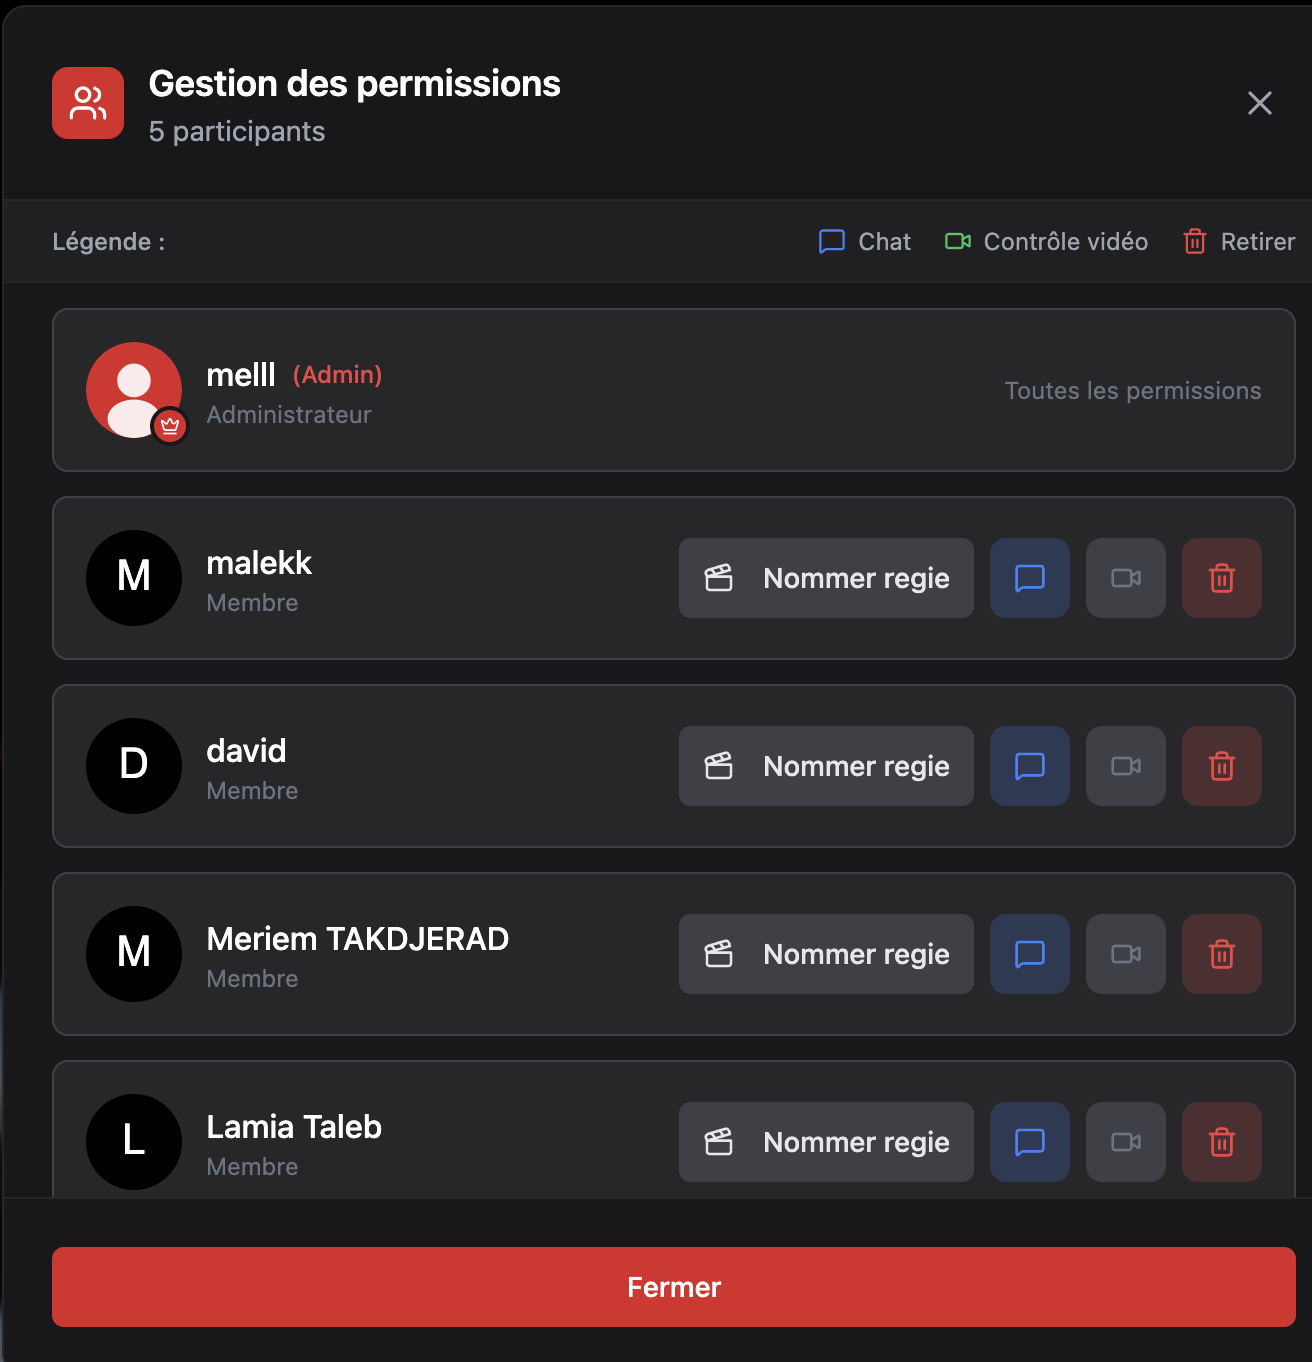
\includegraphics[width=0.8\textwidth]{regie_interface.png}
\caption{Interface de régie vidéo}
\end{figure}

\subsubsection{Gestion des rôles et permissions}

Un système de rôles adapté au contexte universitaire a été mis en place :

\begin{itemize}
  \item \textbf{Professeur :} création de salons et gestion des vidéos ;
  \item \textbf{Régie :} contrôle de la vidéo (lecture, pause, changement) ;
  \item \textbf{Étudiant :} accès en consultation uniquement.
\end{itemize}

Le rôle de régie peut être attribué ou retiré dynamiquement à un utilisateur.
Les permissions sont mises à jour en temps réel et conditionnent l’accès
aux contrôles vidéo.

Des fonctionnalités complémentaires ont été ajoutées :
\begin{itemize}
  \item activation / désactivation du chat ;
  \item restriction des actions selon le rôle ;
  \item gestion dynamique des permissions.
\end{itemize}



\subsubsection{Implémentation de l’authentification}

Un système d’authentification a été mis en place à l’aide de Supabase :

\begin{itemize}
  \item création de comptes utilisateurs ;
  \item connexion sécurisée ;
  \item stockage des rôles en base de données ;
  \item restriction des inscriptions aux emails universitaires.
\end{itemize}

Détails :
\begin{itemize}
  \item validation réelle des emails étudiants (\texttt{@univ-avignon.fr}) ;
  \item utilisation d’adresses Gmail pour tester les comptes enseignants ;
  \item mots de passe sécurisés via hachage.
\end{itemize}

\begin{figure}[h]
\centering
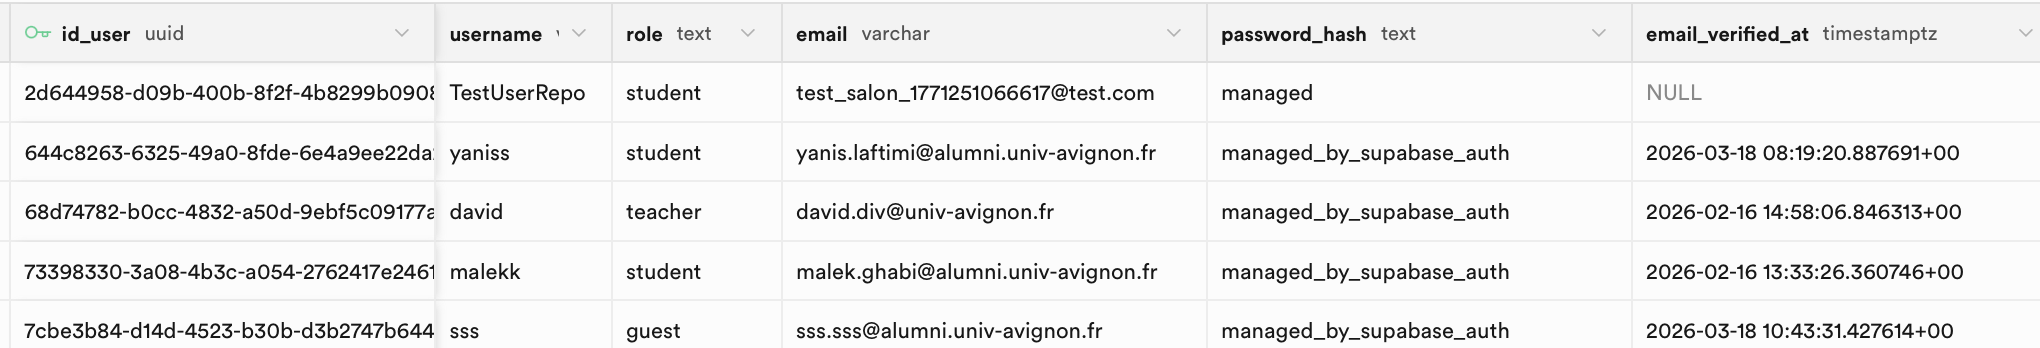
\includegraphics[width=0.7\textwidth]{auth_supabase.png}
\caption{Interface d’authentification}
\end{figure}

\subsubsection{Fonctionnalités liées à la plateforme sécurisée}

Plusieurs mécanismes ont été implémentés ou testés :

\begin{itemize}
  \item distinction entre contenus publics et privés ;
  \item accès à un salon via code d’invitation ou mot de passe ;
  \item ajout d’une filière lors de l’inscription ;
  \item accès différencié aux contenus selon la filière.
\end{itemize}

Ces éléments permettent de structurer l’accès aux contenus pédagogiques.

\subsubsection{Adaptation de l’interface utilisateur}

Une adaptation du design a été initiée afin de mieux correspondre au public
universitaire.

\begin{itemize}
  \item simplification de l’interface ;
  \item affichage des fonctionnalités selon le rôle ;
  \item amélioration de la lisibilité des contenus.
\end{itemize}

\begin{figure}[h]
\centering
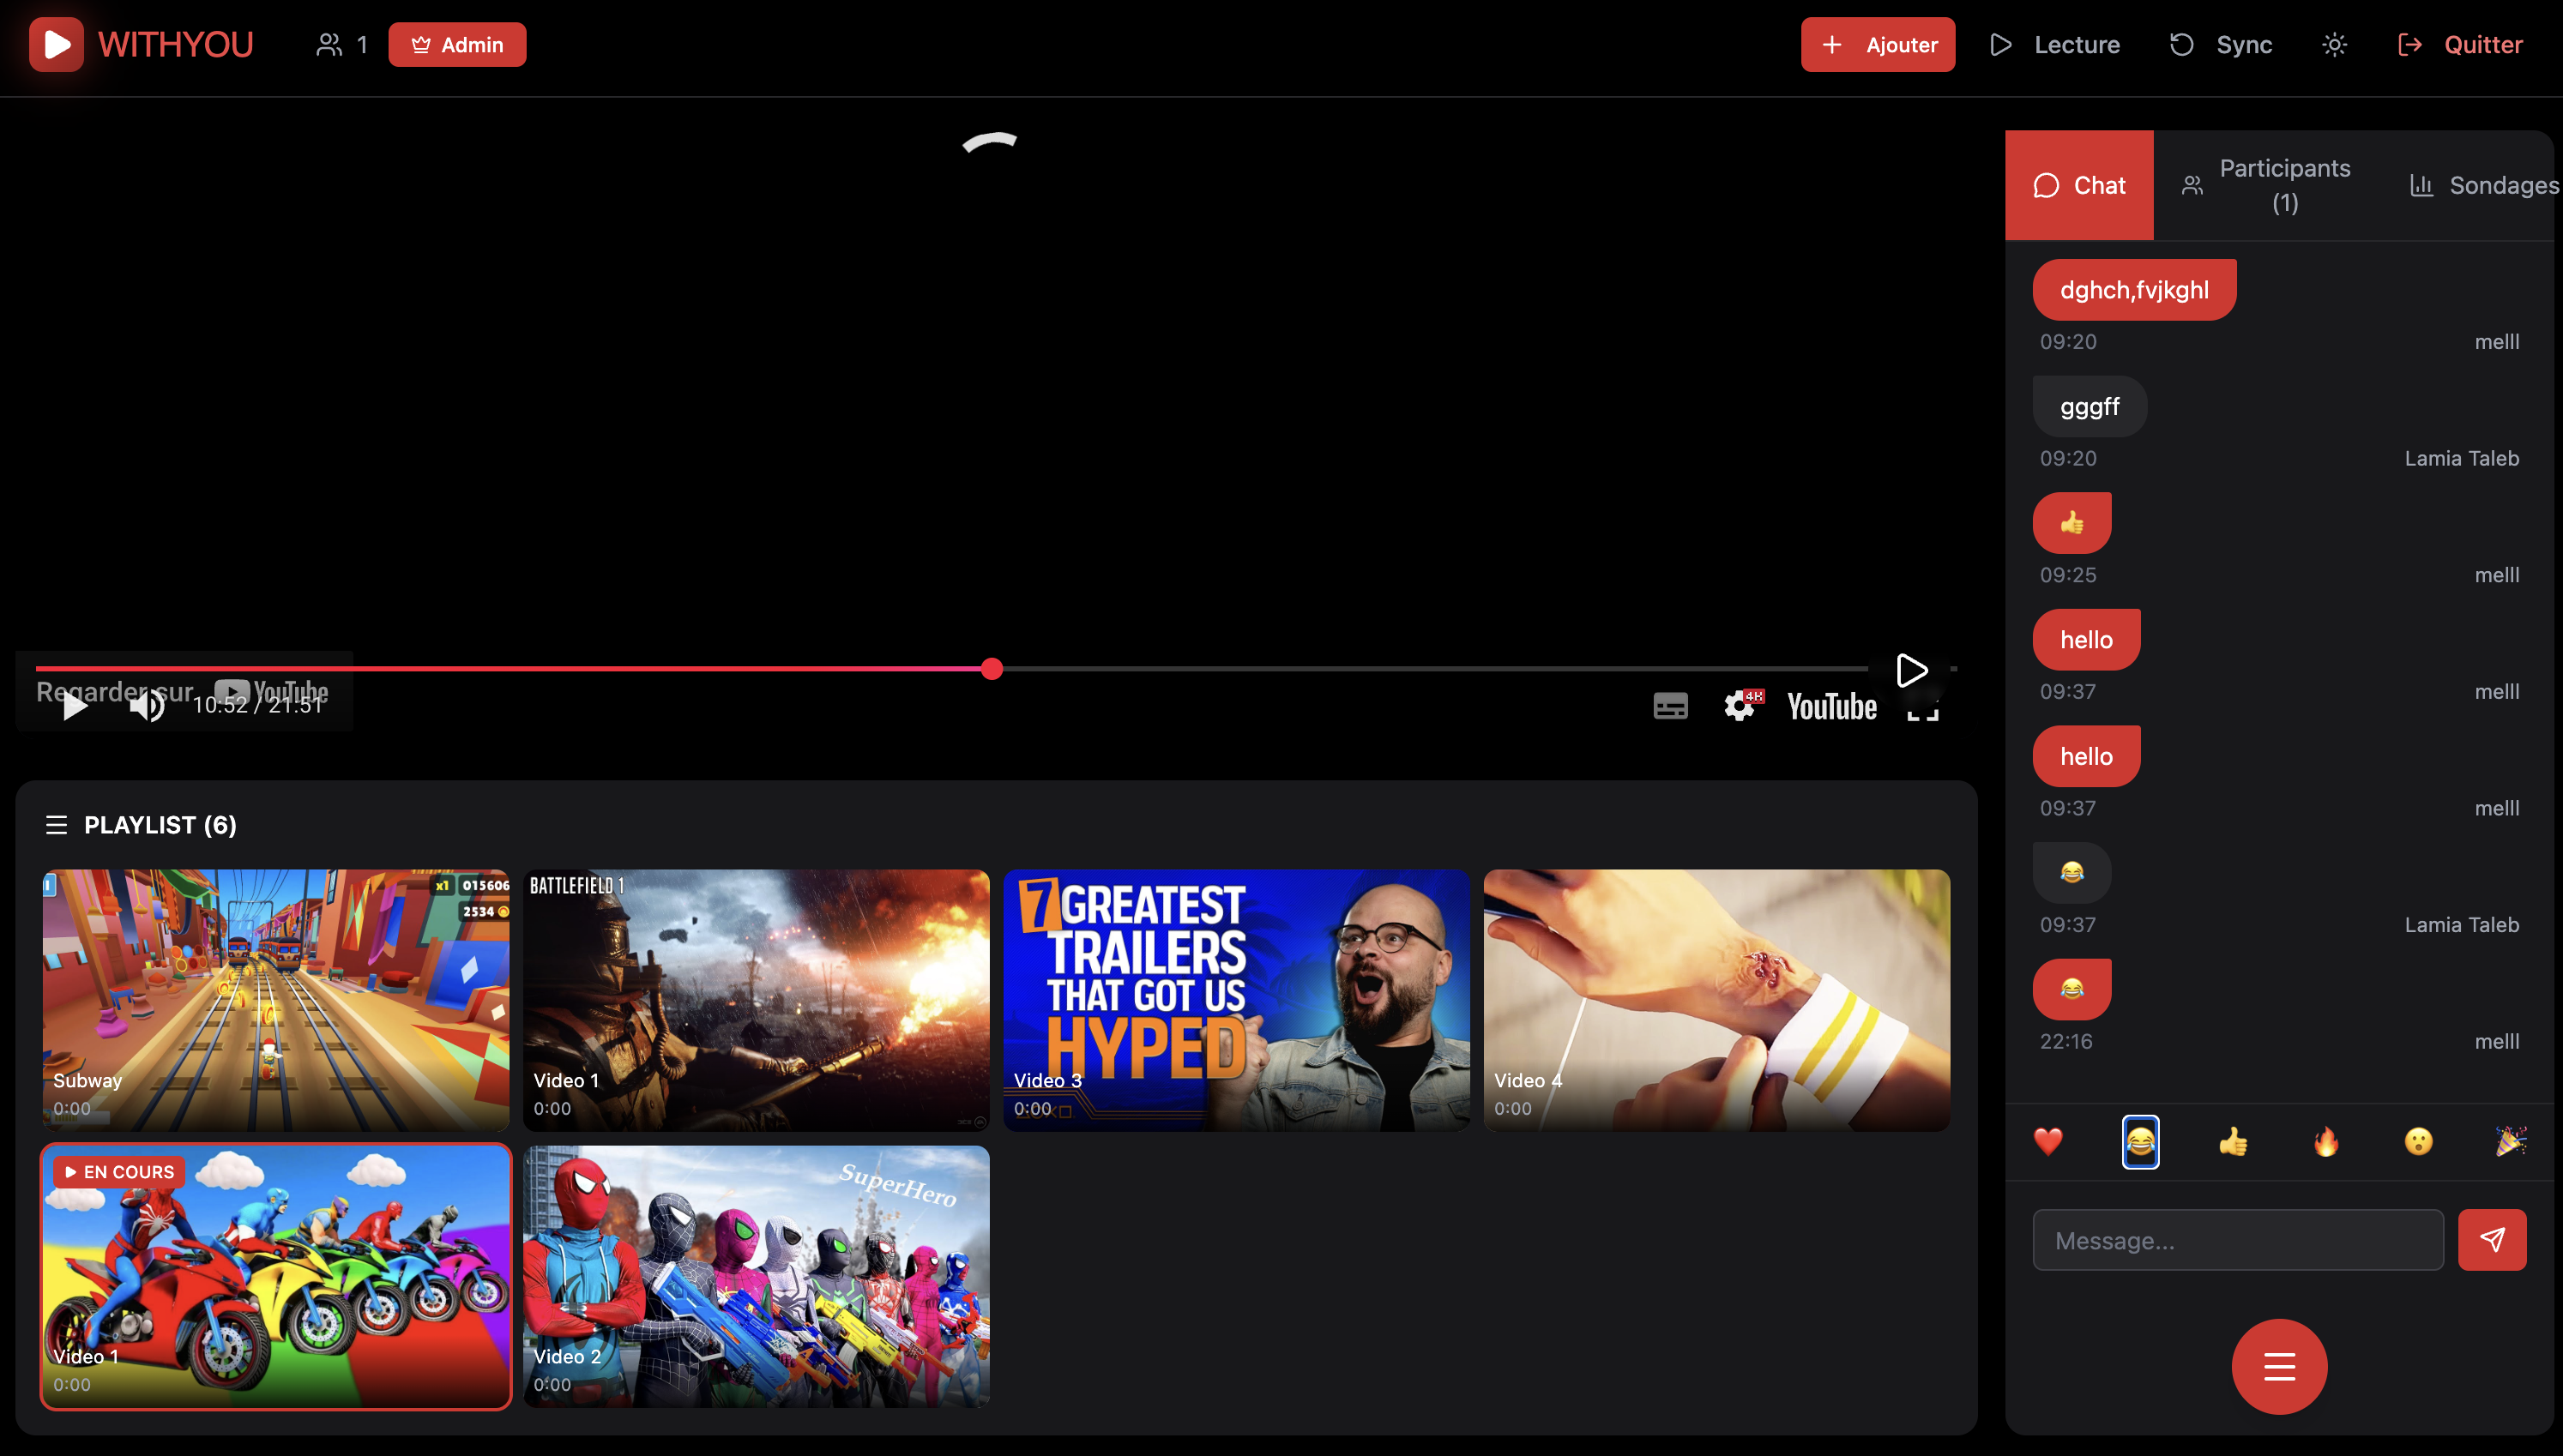
\includegraphics[width=0.8\textwidth]{ui_design.png}
\caption{Adaptation de l’interface utilisateur}
\end{figure}

% ----------------------------------------------------------
\subsection{Tests réalisés}

\begin{itemize}
  \item tests de synchronisation vidéo entre utilisateurs ;
  \item tests des actions de régie (lecture, pause, avance, changement de vidéo) ;
  \item tests des rôles et permissions en temps réel ;
  \item tests de l’authentification et des restrictions d’accès.
\end{itemize}

% ----------------------------------------------------------
\subsection{Résultats et décisions}

\begin{itemize}
  \item la régie vidéo est fonctionnelle et permet un contrôle centralisé ;
  \item la synchronisation est globalement fiable, malgré de légers décalages ;
  \item les fonctionnalités avancées (playlist, navigation) sont opérationnelles ;
  \item la gestion des rôles (étudiant / professeur / régie) est cohérente ;
  \item l’authentification constitue une base solide pour la sécurisation.
\end{itemize}

Ces résultats confirment la faisabilité technique du projet et valident les
choix effectués lors du Cycle 1.

% ----------------------------------------------------------
\subsection{Planification du cycle suivant}

Le Cycle 3 aura pour objectif de finaliser et stabiliser l’application.

\begin{itemize}
  \item amélioration de la synchronisation et réduction des décalages ;
  \item finalisation de la validation des comptes ;
  \item amélioration des rôles et permissions ;
  \item stabilisation globale et correction des bugs.
\end{itemize}

L’objectif final est de produire une version stable, sécurisée et utilisable
de la plateforme.

% =========================
% Cycle 3 – Implémentation finale (à venir)
% =========================
\chapter{Cycle 3 – Implémentation finale (à venir)}
Cette section détaillera l’implémentation finale, les optimisations réalisées et le bilan critique du projet.

% =========================
% Conclusion
% =========================
\chapter{Conclusion}

Le Cycle 1 a permis d’identifier, comparer et analyser trois pistes d’évolution pour la plateforme WithYou, en mettant en évidence les risques associés à chacune d’elles.

À l’issue de cette analyse, la stratégie retenue repose principalement sur la mise en place d’une régie vidéo avancée, complétée par une structuration progressive vers une plateforme de formation sécurisée.

Le Cycle 2 a permis de valider la faisabilité technique de ces choix à travers un prototype fonctionnel, notamment en ce qui concerne la synchronisation vidéo, la gestion des rôles, l’authentification et l’adaptation de l’interface au public universitaire.

Le Cycle 3 permettra de finaliser l’application, d’améliorer sa stabilité et de proposer une version complète, cohérente et adaptée au public visé.

\end{document}